\documentclass[11pt]{article}

\usepackage[margin=0.85in]{geometry}
\usepackage[T1]{fontenc}
\usepackage{lmodern}
\usepackage{microtype}
\usepackage{xcolor}
\usepackage{graphicx}
\usepackage{amsmath}
\usepackage{booktabs}
\usepackage{tabularx}
\usepackage{array}
\usepackage{caption}
\usepackage{float}
\usepackage{placeins}
\usepackage[round]{natbib}
\usepackage[hidelinks]{hyperref}

\definecolor{navy}{HTML}{102A43}
\definecolor{muted}{HTML}{526173}
\definecolor{fieldgreen}{HTML}{86D973}
\definecolor{goalblue}{HTML}{155E9E}
\definecolor{turnoverred}{HTML}{B43F35}

\newcolumntype{Y}{>{\raggedright\arraybackslash}X}
\newcommand{\aEC}{aEC}
\newcommand{\pos}{possession}
\newcommand{\Oline}{O-line}
\newcommand{\Dline}{D-line}

\title{\textcolor{navy}{Deep Hucks or Small Ball?}\\[4pt]
  \large Common Offensive Possession Patterns Among Four 2026 UFA Semifinalists}
\author{Team-level spatial analysis of UFA play-by-play data}
\date{August 2026}

\begin{document}
\maketitle

\begin{abstract}
Professional ultimate possessions are often summarized by their endpoint: a goal,
a turnover, or a break. That summary leaves out the route. This paper examines
the repeated spatial routes used by the New York Empire, Austin Sol, Minnesota
Wind Chill, and Oakland Spiders during the 2026 regular season. We combine
throw-level Shown Space data with manually curated field-path groups, then
describe each selected pattern using frequency, goal/turnover efficiency, total
\aEC per possession, \aEC per throw, and throw count. The result is a team-centered
view of offensive identity. The same outcome can emerge from a short, aggressive
sequence, a longer reset-heavy possession, or a low-huck path that steadily
compresses the field. A league-wide throw-count heatmap provides the broader
context: five throws is the modal length of an \Oline goal possession, but the
four teams examined here occupy noticeably different parts of that distribution.
\end{abstract}

\section{Introduction}

The modern UFA analytics conversation has moved well beyond the final line in a
box score. Shown Space was introduced as a way to use the league's play-by-play
infrastructure to ask how possessions develop, which actions change scoring
probability, and which players drive that change \citep{eberhard2026shownspace}.
That shift matters because two possessions can finish in the same end zone while
asking very different questions of an offense. One may win through immediate
field position and a deep release; another may survive several resets before a
cut finally opens the goal line.

The Sloan work behind Shown Space established a related foundation by combining
machine learning with completion probability and field value to estimate player
decision-making in professional ultimate \citep{eberhard2025sloan}. The public
articles that followed use that foundation as a storytelling device. In the
six-passer comparison, for example, aEC is paired with complementary measures so
that distinct jobs remain visible rather than being flattened into one ranking
\citep{eberhard2026passers}. The lesson transfers naturally from players to
teams: a leaderboard can identify who is productive, while paths can help explain
what that productivity looks like.

This paper applies that idea to the four UFA semifinalists represented in the
current possession browser. The question is deliberately narrower than ``Which
team is best?'' We ask: \emph{What are the recurring spatial forms of each team's
offense, and how do their outcomes and aEC values differ?} The answer should not
be reduced to a single style label. The UFA's own team analysis emphasizes that
the O-line and D-line can become meaningfully different teams after the disc
changes hands, and that a deep ball is a tool rather than a complete offensive
identity \citep{eberhard2026teamstrengths}. Our analysis therefore stays with
\Oline possessions, includes both goals and turnovers, and treats spatial
organization as evidence to be inspected rather than a substitute for judgment.

\section{Data and Methods}

\subsection{Sample and possession reconstruction}

The analysis uses the cached per-game Shown Space throw files in this project.
The regular-season window runs from April 24 through July 19, 2026. The cache
also contains later playoff files, so the figure-building script excludes games
dated after July 19 before calculating any count, efficiency, or aEC statistic.
Each focus team contributes 12 regular-season games. The resulting reconstructed
\Oline samples are 257 possessions for New York, 285 for Austin, 266 for
Minnesota, and 266 for Oakland.

A possession is formed by grouping throws with the same game, quarter, point,
possession number, and home/away side. The final throw determines the outcome:
the two retained outcomes are `goal' and `turnover'. The line type comes from
the source \texttt{o\_line} field. For every possession, the pipeline retains
the ordered throw path, starting and ending field coordinates, throw count,
field progress, huck count, reset count, throw-level \aEC, and the derived
possession totals.

The word ``efficiency'' has a deliberately local meaning in this paper. For a
group of reconstructed \Oline possessions, it is
\[
  \mathrm{efficiency} =
  \frac{\text{goals}}{\text{goals}+\text{turnovers}}.
\]
It is therefore an outcome ratio for this sample, not a claim that it is
identical to the UFA's published OE or expectation-adjusted OEOE measures.
Keeping that distinction explicit is essential when comparing a custom browser
view with a public leaderboard.

\subsection{Human-in-the-loop spatial grouping}

The first three rows in each saved arrangement checkpoint
(\texttt{data/arrangements/2026/empire.json}, \texttt{sol.json},
\texttt{windchill.json}, and \texttt{spiders.json}) are treated as that team's
three selected recurring patterns. The grouping was made by reviewing field
cards and overlaying paths, then deciding which routes were similar enough to
share a row. This is a manual taxonomy with a reproducible checkpoint, not an
unsupervised claim that the game contains exactly three natural clusters.

For the paper, a card contributes to a pattern's statistics only when its
possession is in the regular-season data and its line type is \Oline. The field
figures draw every retained path in a selected group, with goals in blue and
turnovers in red. That choice keeps the display honest: a group can look
spatially coherent while still containing different outcomes.

\subsection{Metrics}

For a pattern $g$ with $n_g$ possessions and $T_g$ total throws, we report:

\begin{itemize}
  \item \textbf{frequency}: $n_g/N_t$, where $N_t$ is the team's regular-season
        \Oline possession count;
  \item \textbf{efficiency}: the goal fraction defined above, with turnovers in
        the denominator;
  \item \textbf{total \aEC per possession}: $\sum aEC/n_g$;
  \item \textbf{\aEC per throw}: $\sum aEC/T_g$; and
  \item \textbf{median throws}: the median number of throws in the pattern.
\end{itemize}

The throw-level \aEC values are taken from the cached Shown Space rows and
summed within each possession. We do not normalize a pattern to equal one or
discard negative values. As a result, a successful possession often lands near
one total \aEC, while a turnover can pull the total below zero; the average is
intended to preserve that outcome-sensitive signal. Reporting both total \aEC
per possession and \aEC per throw also prevents a short possession from being
mistaken for a high-volume one.

\section{Results}

\subsection{The league context: five throws is common, not destiny}

Figure~\ref{fig:heatmap} shows the throw-count distribution for regular-season
\Oline goal possessions across all 22 cached teams. Each row is normalized within
team, so the darkest cell answers a within-team question: which throw count
appears most often among that team's goals? Across the league, the mode is five
throws among 3,607 \Oline goal possessions. The focus teams do not share that
mode. Austin peaks at four throws; Oakland and Minnesota peak at eight; New York
peaks at nine. A mode describes the most frequent length, not an offensive
instruction. It is best read alongside the rest of the row, especially when two
nearby counts have similar mass.

\begin{figure}[p]
  \centering
  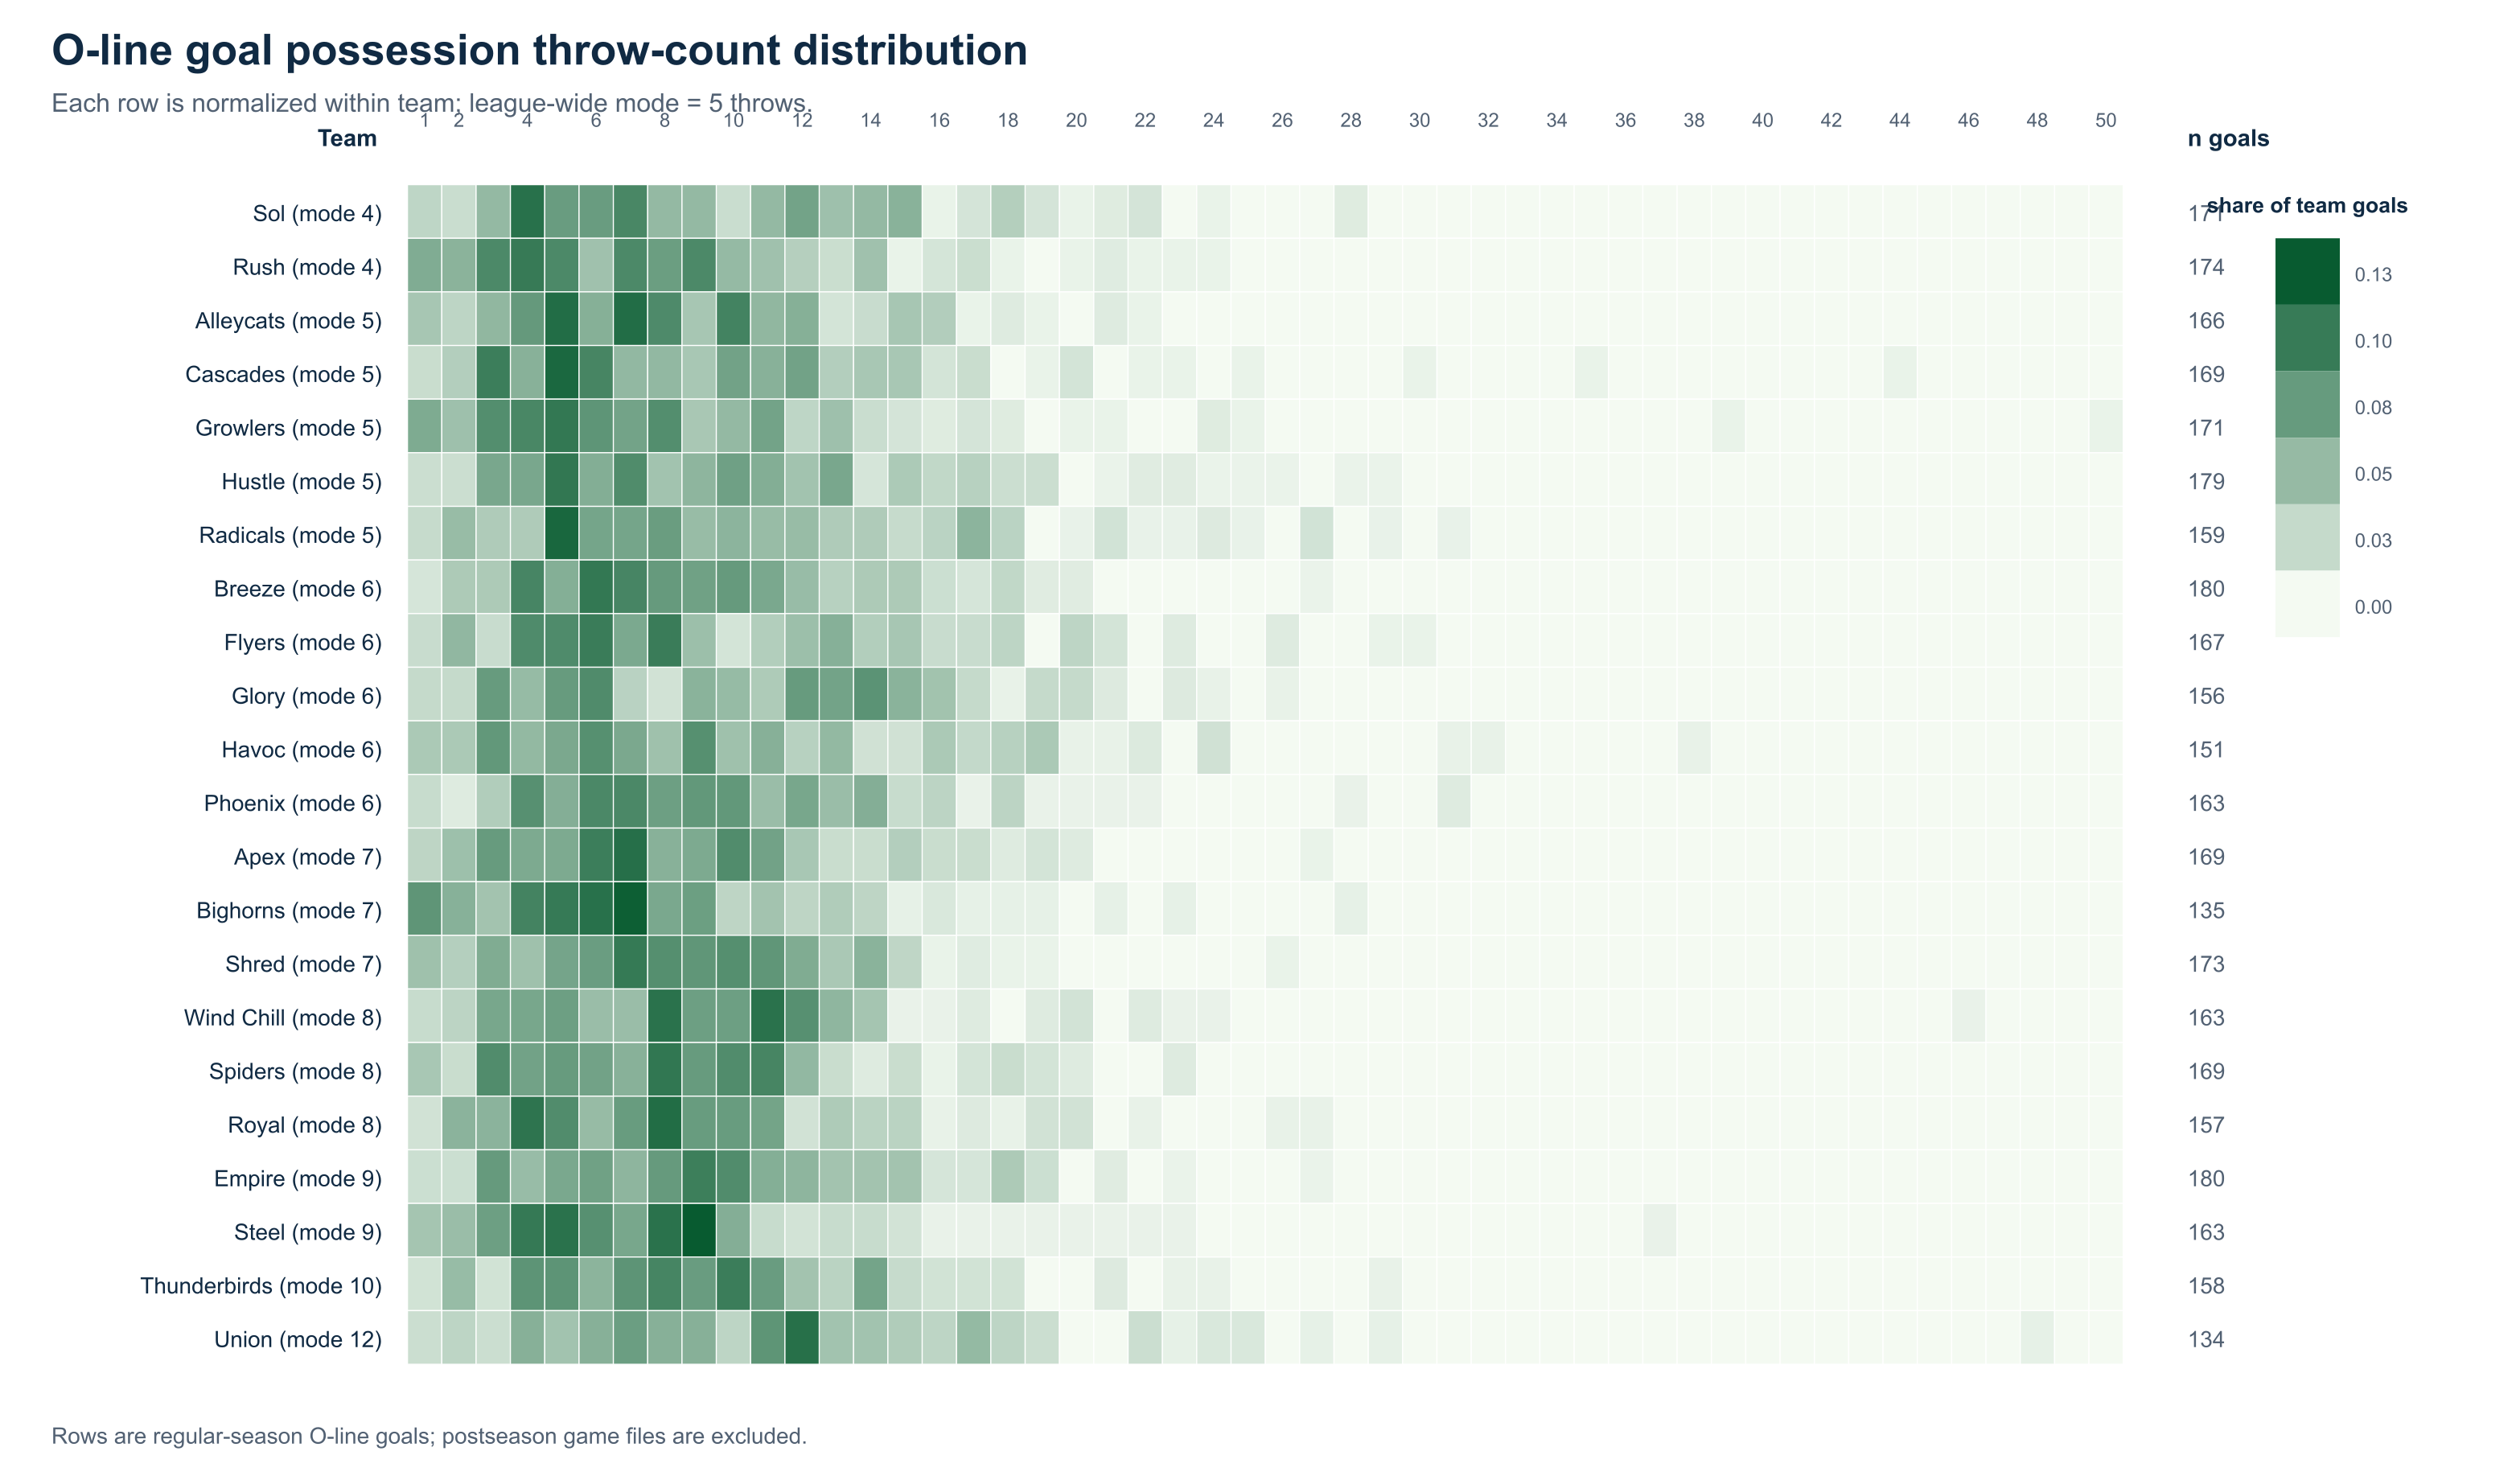
\includegraphics[width=0.98\linewidth]{generated/figures/league_throw_count_heatmap.png}
  \caption{Regular-season throw-count distribution for \Oline goal possessions.
  Color is the share of each team's \Oline goals, not the share of all league
  possessions. The right-hand count is the number of goal possessions used for
  that row.}
  \label{fig:heatmap}
\end{figure}

\subsection{Team-level baseline}

The four teams separate before the individual patterns are considered
(Table~\ref{tab:team-summary}). New York's reconstructed \Oline converted 180
of 257 possessions, or 70.0 percent. Oakland followed at 63.5 percent, while
Minnesota and Austin finished at 61.3 and 60.0 percent, respectively. New York
also led this local sample in average total \aEC per possession (0.592) and
aggregate \aEC per throw (0.070). Those values should be interpreted as
descriptive summaries of the cached rows, not as a replacement for the public
Shown Space team metrics.

\begin{table}[H]
  \centering
  \caption{Regular-season reconstructed \Oline baseline.}
  \label{tab:team-summary}
  \small
  \begin{tabular}{lrrrrrrr}
    \toprule
    Team & Games & Pos. & Goals & TOs & Eff. & aEC/pos. & aEC/throw \\
    \midrule
    New York Empire & 12 & 257 & 180 & 77 & 70.0\% & 0.592 \\
Austin Sol & 12 & 285 & 171 & 114 & 60.0\% & 0.431 \\
Minnesota Wind Chill & 12 & 266 & 163 & 103 & 61.3\% & 0.486 \\
Oakland Spiders & 12 & 266 & 169 & 97 & 63.5\% & 0.492 \\
\bottomrule

  \end{tabular}
\end{table}

\subsection{New York Empire: deep options inside a highly efficient base}

The Empire's first selected pattern is also its largest of the three selected
rows.
After the regular-season and \Oline filters, it contains 25 possessions: 23
goals and two turnovers, for 92.0 percent efficiency. Its median length is six
throws, and 60.0 percent of the possessions contain a huck. The second and third
patterns are smaller, but both converted every retained possession. Pattern 2
is the most compressed value profile of the three, with 0.224 \aEC per throw
across a five-throw median. Pattern 3 reaches the highest average total \aEC per
possession (1.049) while taking a nine-throw median.

That combination suggests an offense with multiple ways to finish a full-field
attack. The short pattern is not merely a quick score, and the longer pattern
is not automatically less valuable. They differ in how densely value is
created, which is precisely why total \aEC and \aEC per throw belong in the same
conversation. This echoes the broader UFA description of New York as a high-
completion offense whose strength comes from the quality of its decisions, not
from avoiding every aggressive option \citep{eberhard2026teamstrengths}.

\begin{figure}[p]
  \centering
  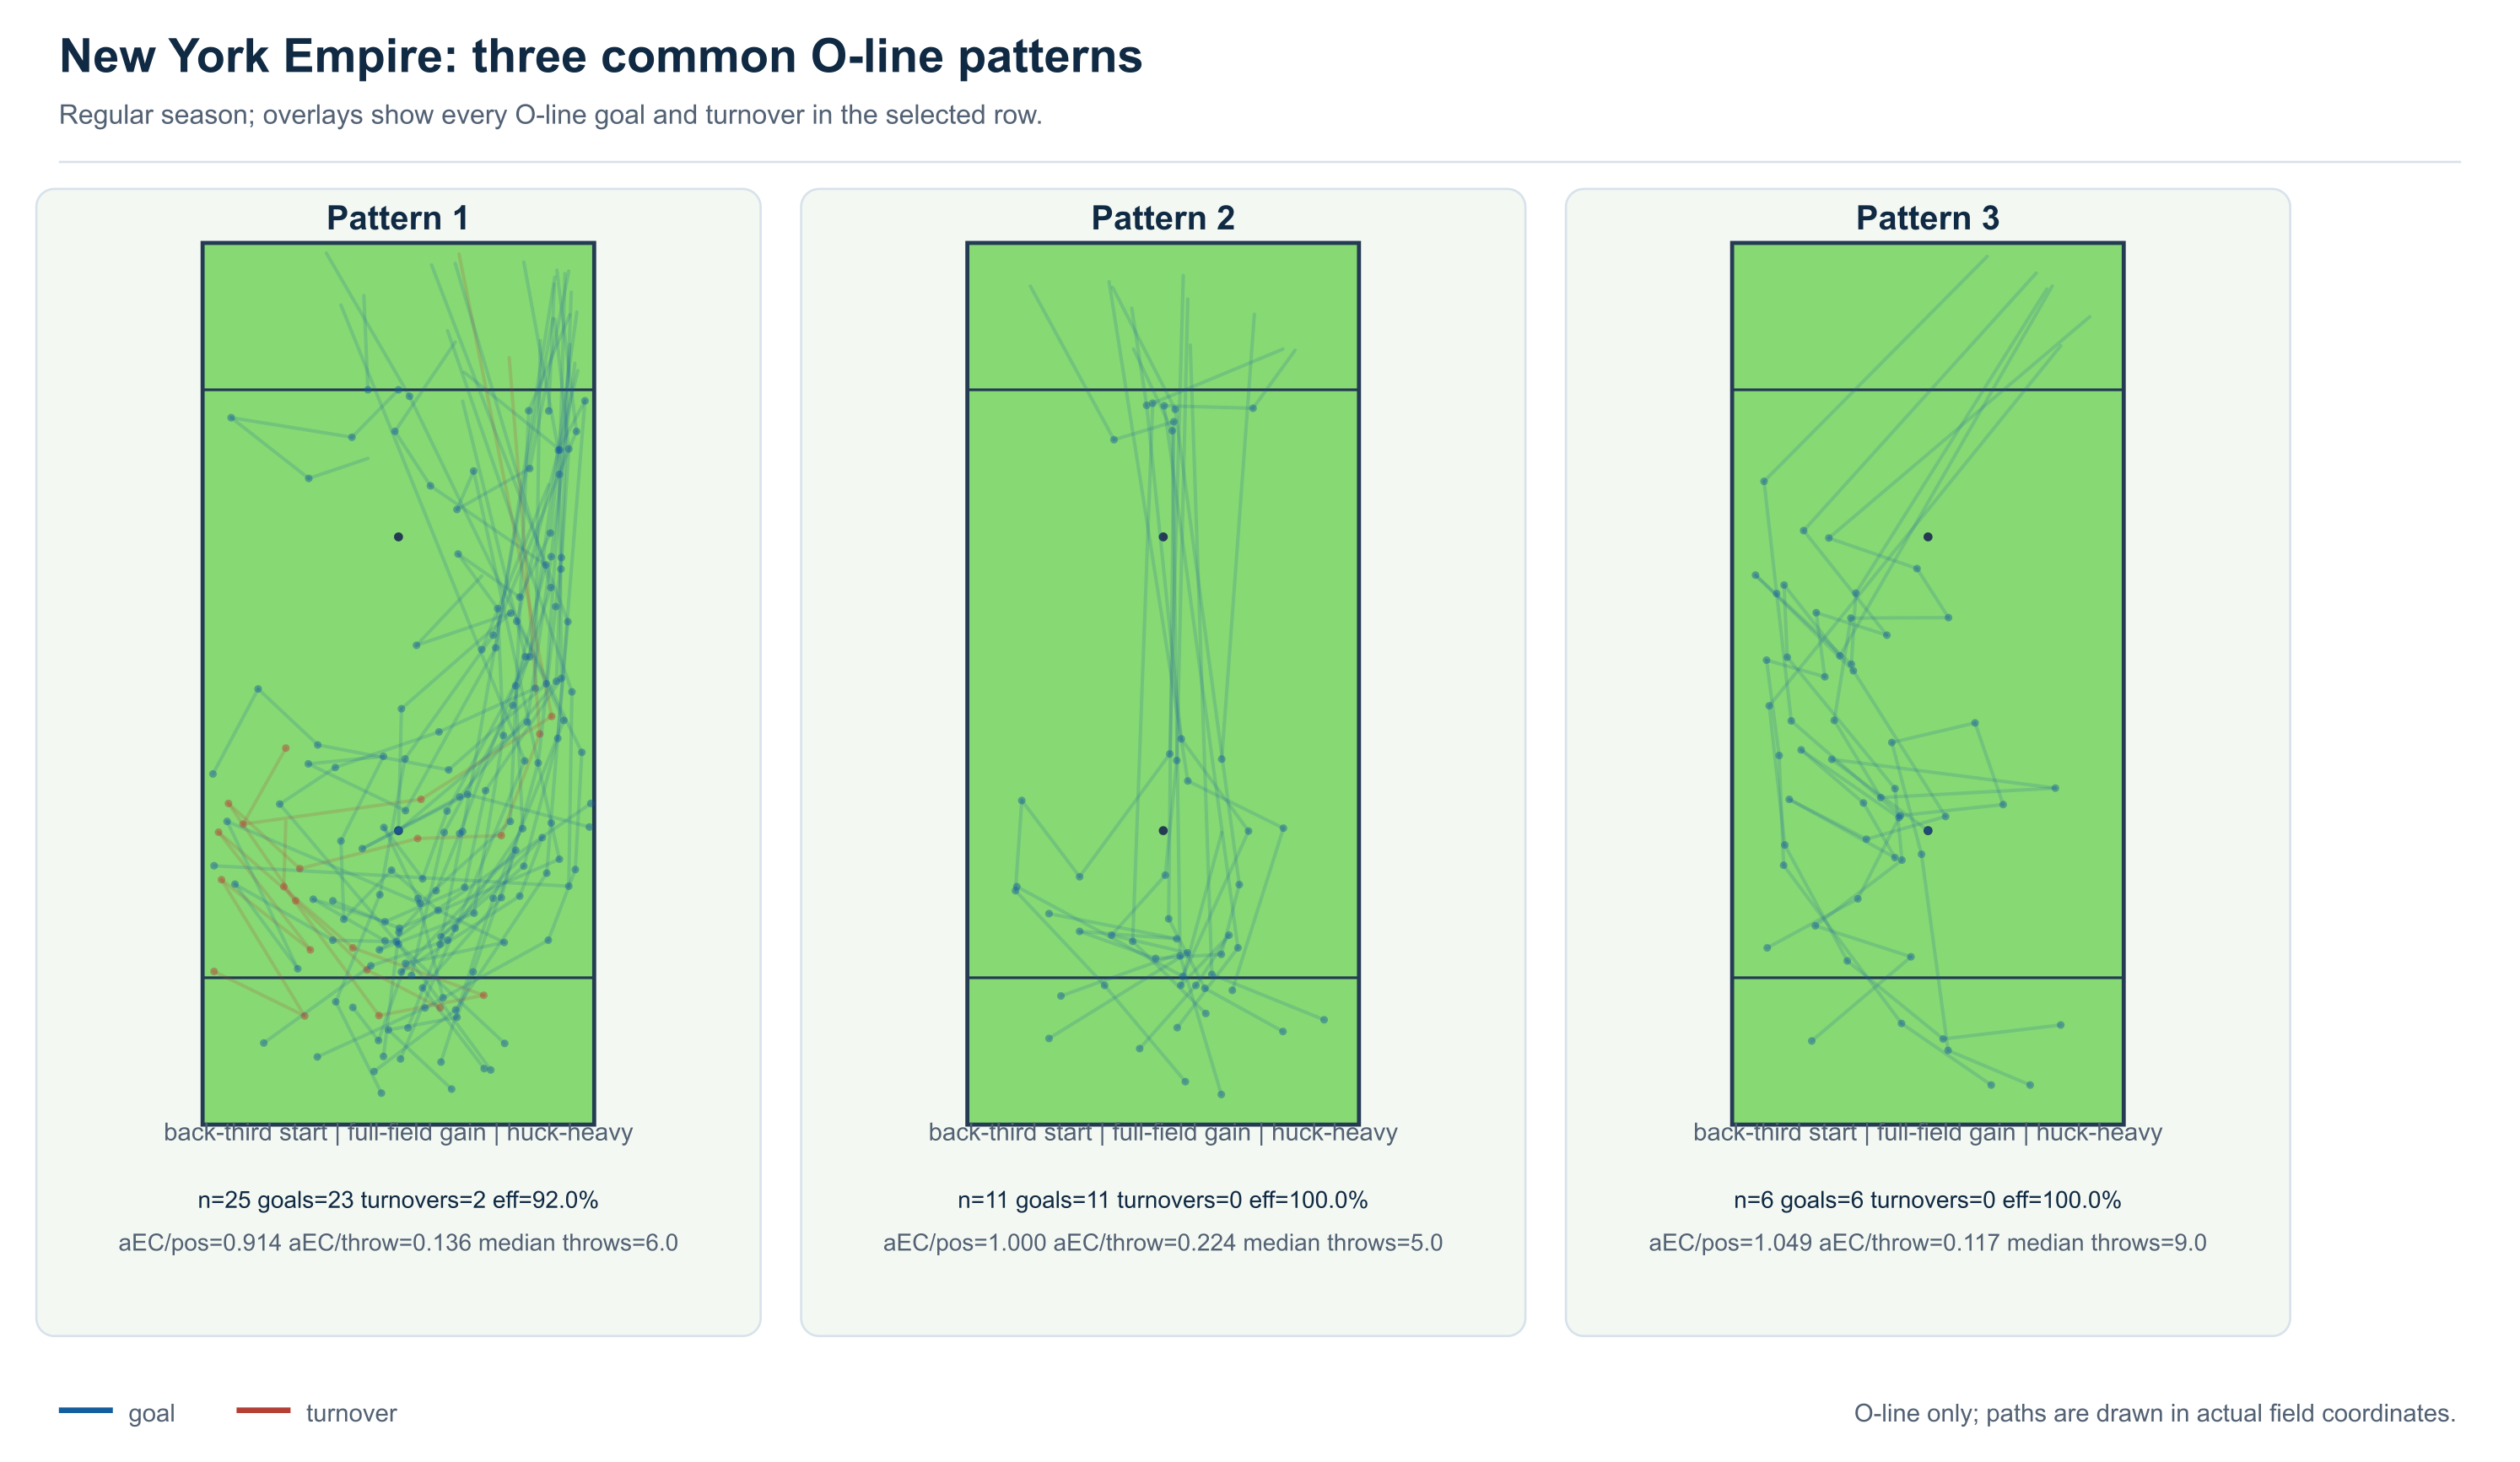
\includegraphics[width=0.98\linewidth]{generated/figures/empire_top3_patterns.png}
  \caption{New York Empire's three selected recurring patterns. Each field
  overlays the regular-season \Oline paths retained in that row; blue is a goal
  and red is a turnover. The metrics below each field include both outcomes.}
  \label{fig:empire}
\end{figure}

\subsection{Austin Sol: a fast branch and two longer answers}

Austin's three selected rows reveal a different balance. Pattern 1 is the
shortest, with a four-throw median and a 100 percent huck rate, but its 11
possessions converted at 72.7 percent. Pattern 2 is more frequent (19
possessions) and longer (10 throws at the median), while Pattern 3 begins from
a more advanced field position and has the highest efficiency of the three at
83.3 percent. The longer two patterns account for 37 selected regular-season
possessions and together show that a Sol attack can keep working after the
first high-value option disappears.

The aEC numbers reinforce that contrast. Pattern 1 creates value most densely
(0.132 per throw), whereas Pattern 3 produces the largest average total among
the three (0.876 per possession). A single ranking would make one of those
facts disappear. The public UFA writing makes a similar move when it separates
team identity from a single efficiency number and emphasizes how a unit gets to
its finishing chances \citep{eberhard2026teamstrengths}.

\begin{figure}[p]
  \centering
  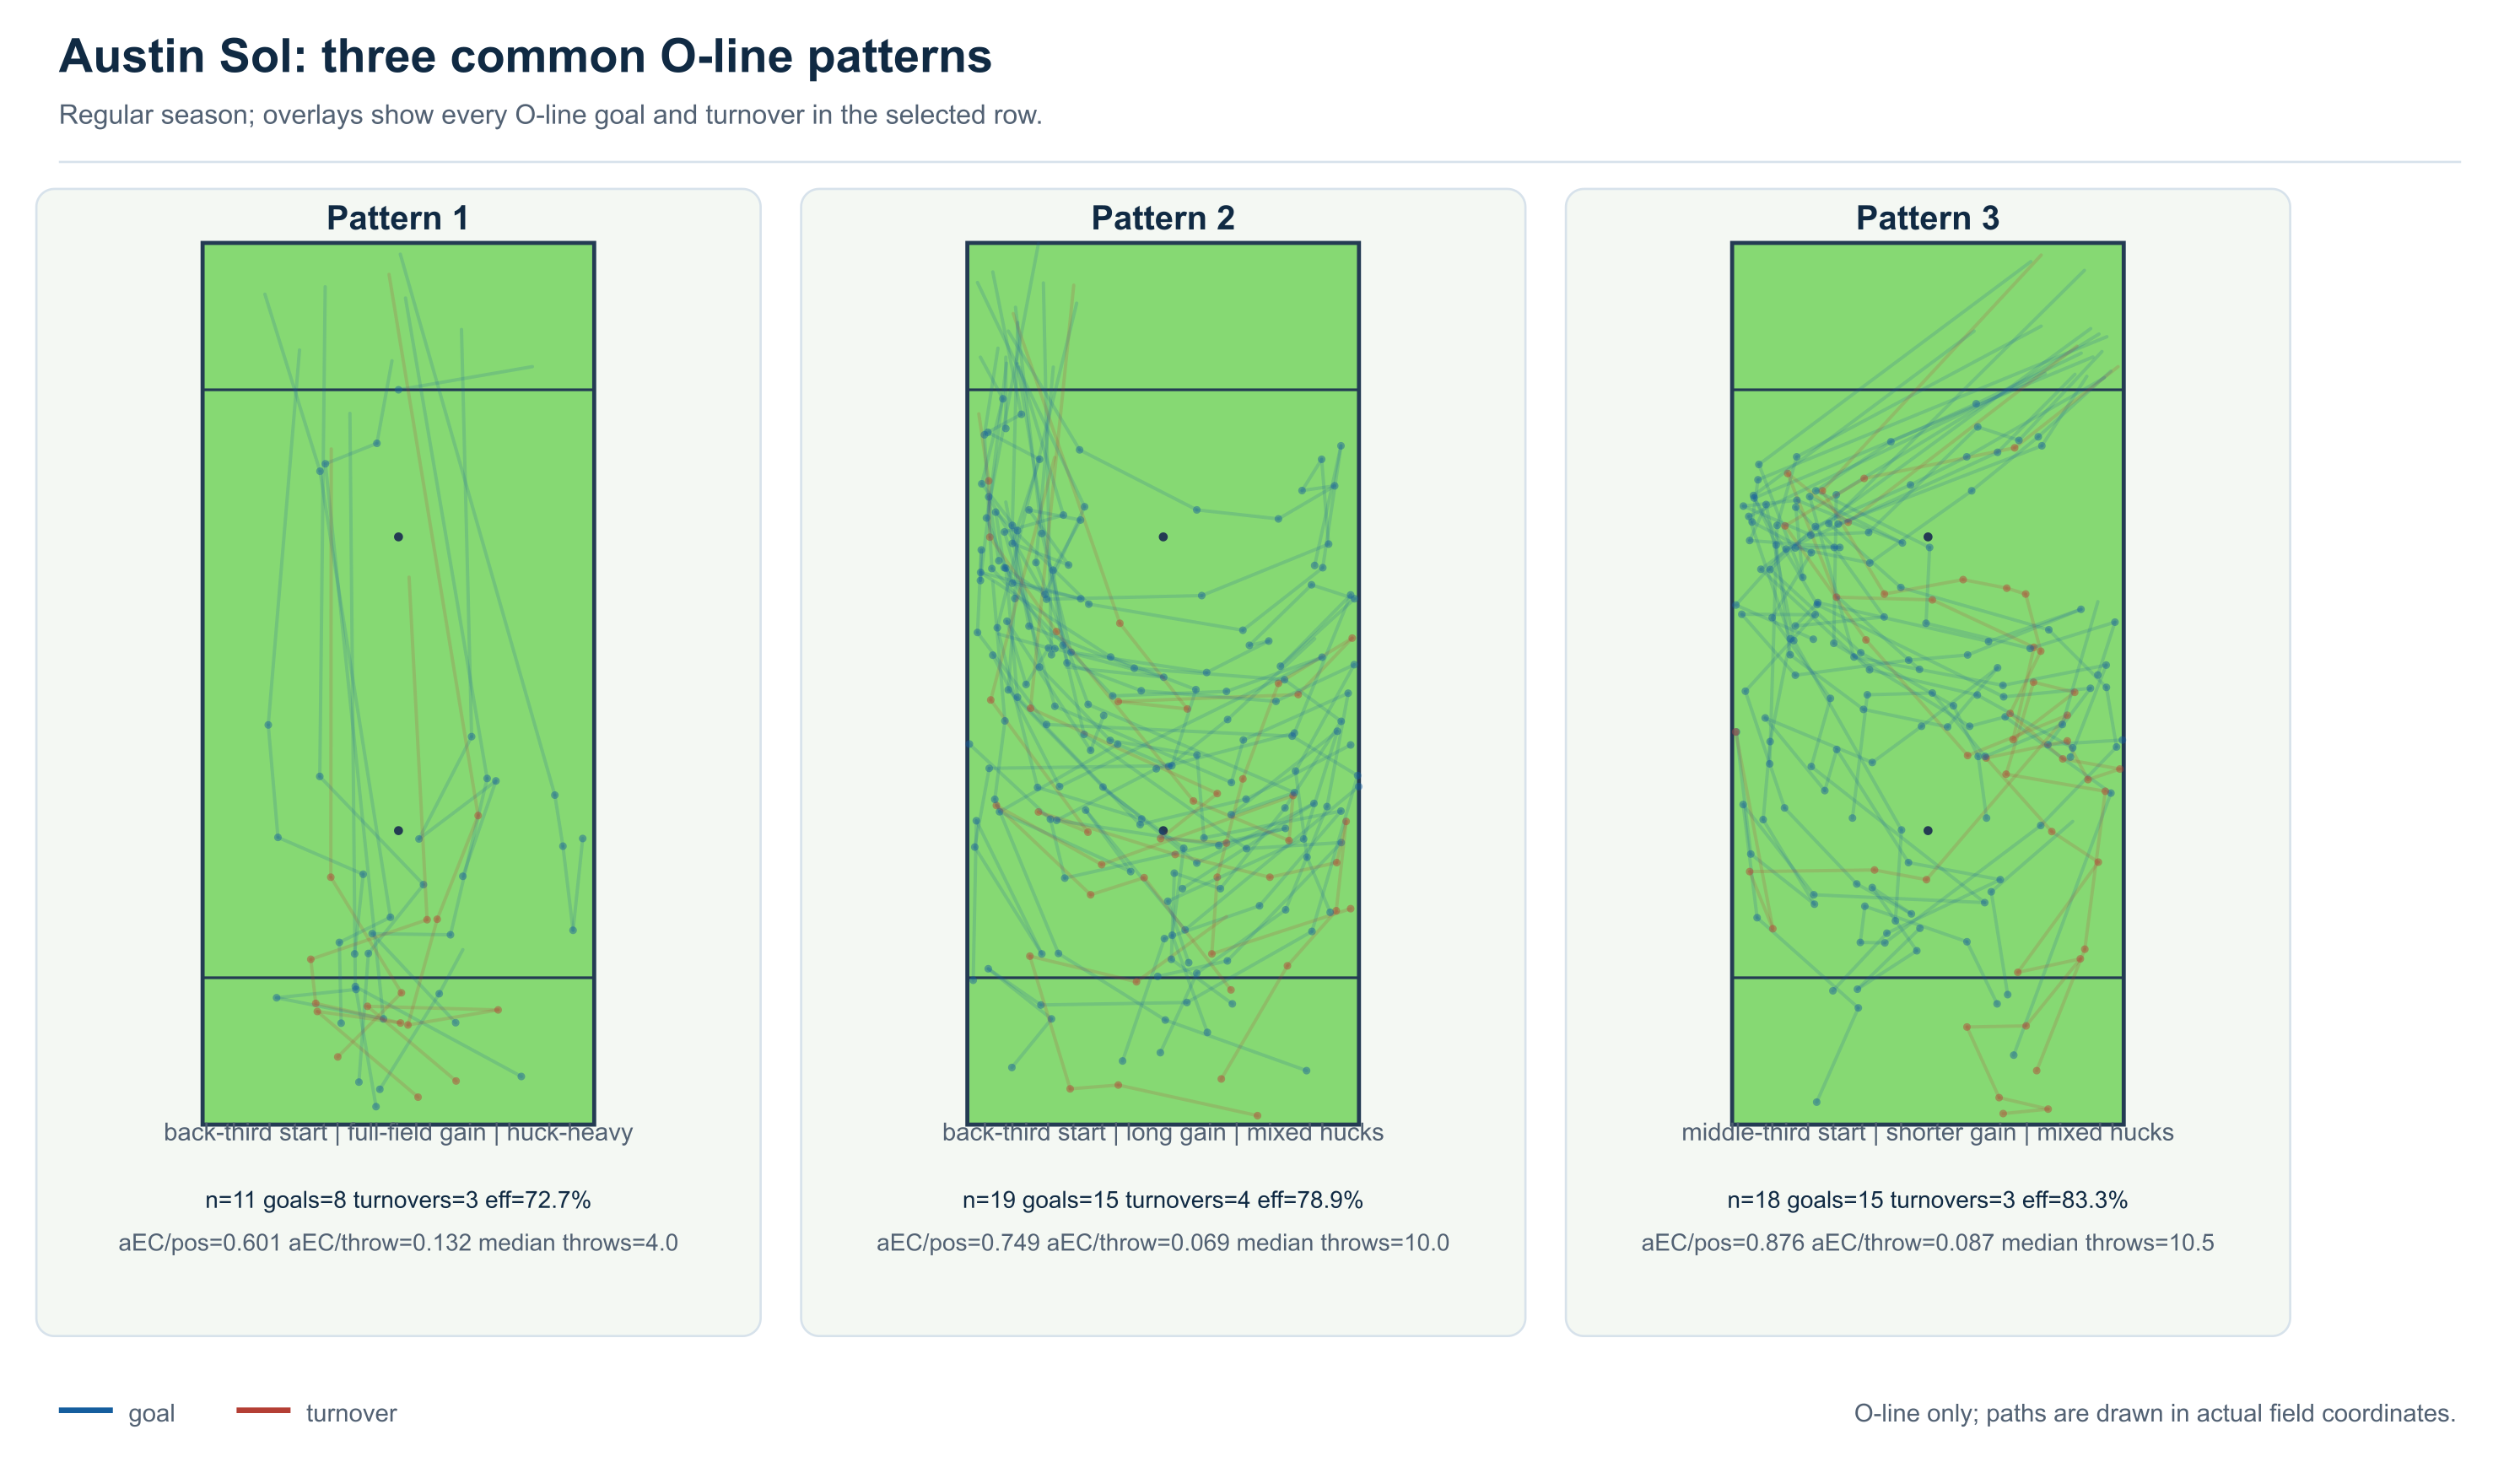
\includegraphics[width=0.98\linewidth]{generated/figures/sol_top3_patterns.png}
  \caption{Austin Sol's three selected recurring patterns. The selected rows
  include both goal and turnover paths; the sample size beneath each field keeps
  the apparent 100 percent or near-100 percent rates in context.}
  \label{fig:sol}
\end{figure}

\subsection{Minnesota Wind Chill: a repeatable middle with small high-value branches}

Minnesota's first pattern is the meaningful base of its selected set: 17
possessions, an eight-throw median, 76.5 percent efficiency, and 0.671 total
\aEC per possession. Patterns 2 and 3 are much smaller, with five and two
possessions, respectively, and both finished without a turnover in this sample.
Their perfect rates should be read as evidence about the observed cards, not as
stable estimates of the team's true conversion probability. Pattern 3's 1.071
total \aEC per possession is attractive, but it is supported by only two
regular-season possessions.

The spatial story is therefore one of a common middle path surrounded by
specialized branches. Minnesota's modal goal length is eight throws, and the
selected patterns mostly sit near eight to ten throws. That aligns with the
broader observation that modern UFA offenses can trade frequent deep attempts
for longer possessions and more deliberate progression \citep{eberhard2026smallball}.

\begin{figure}[p]
  \centering
  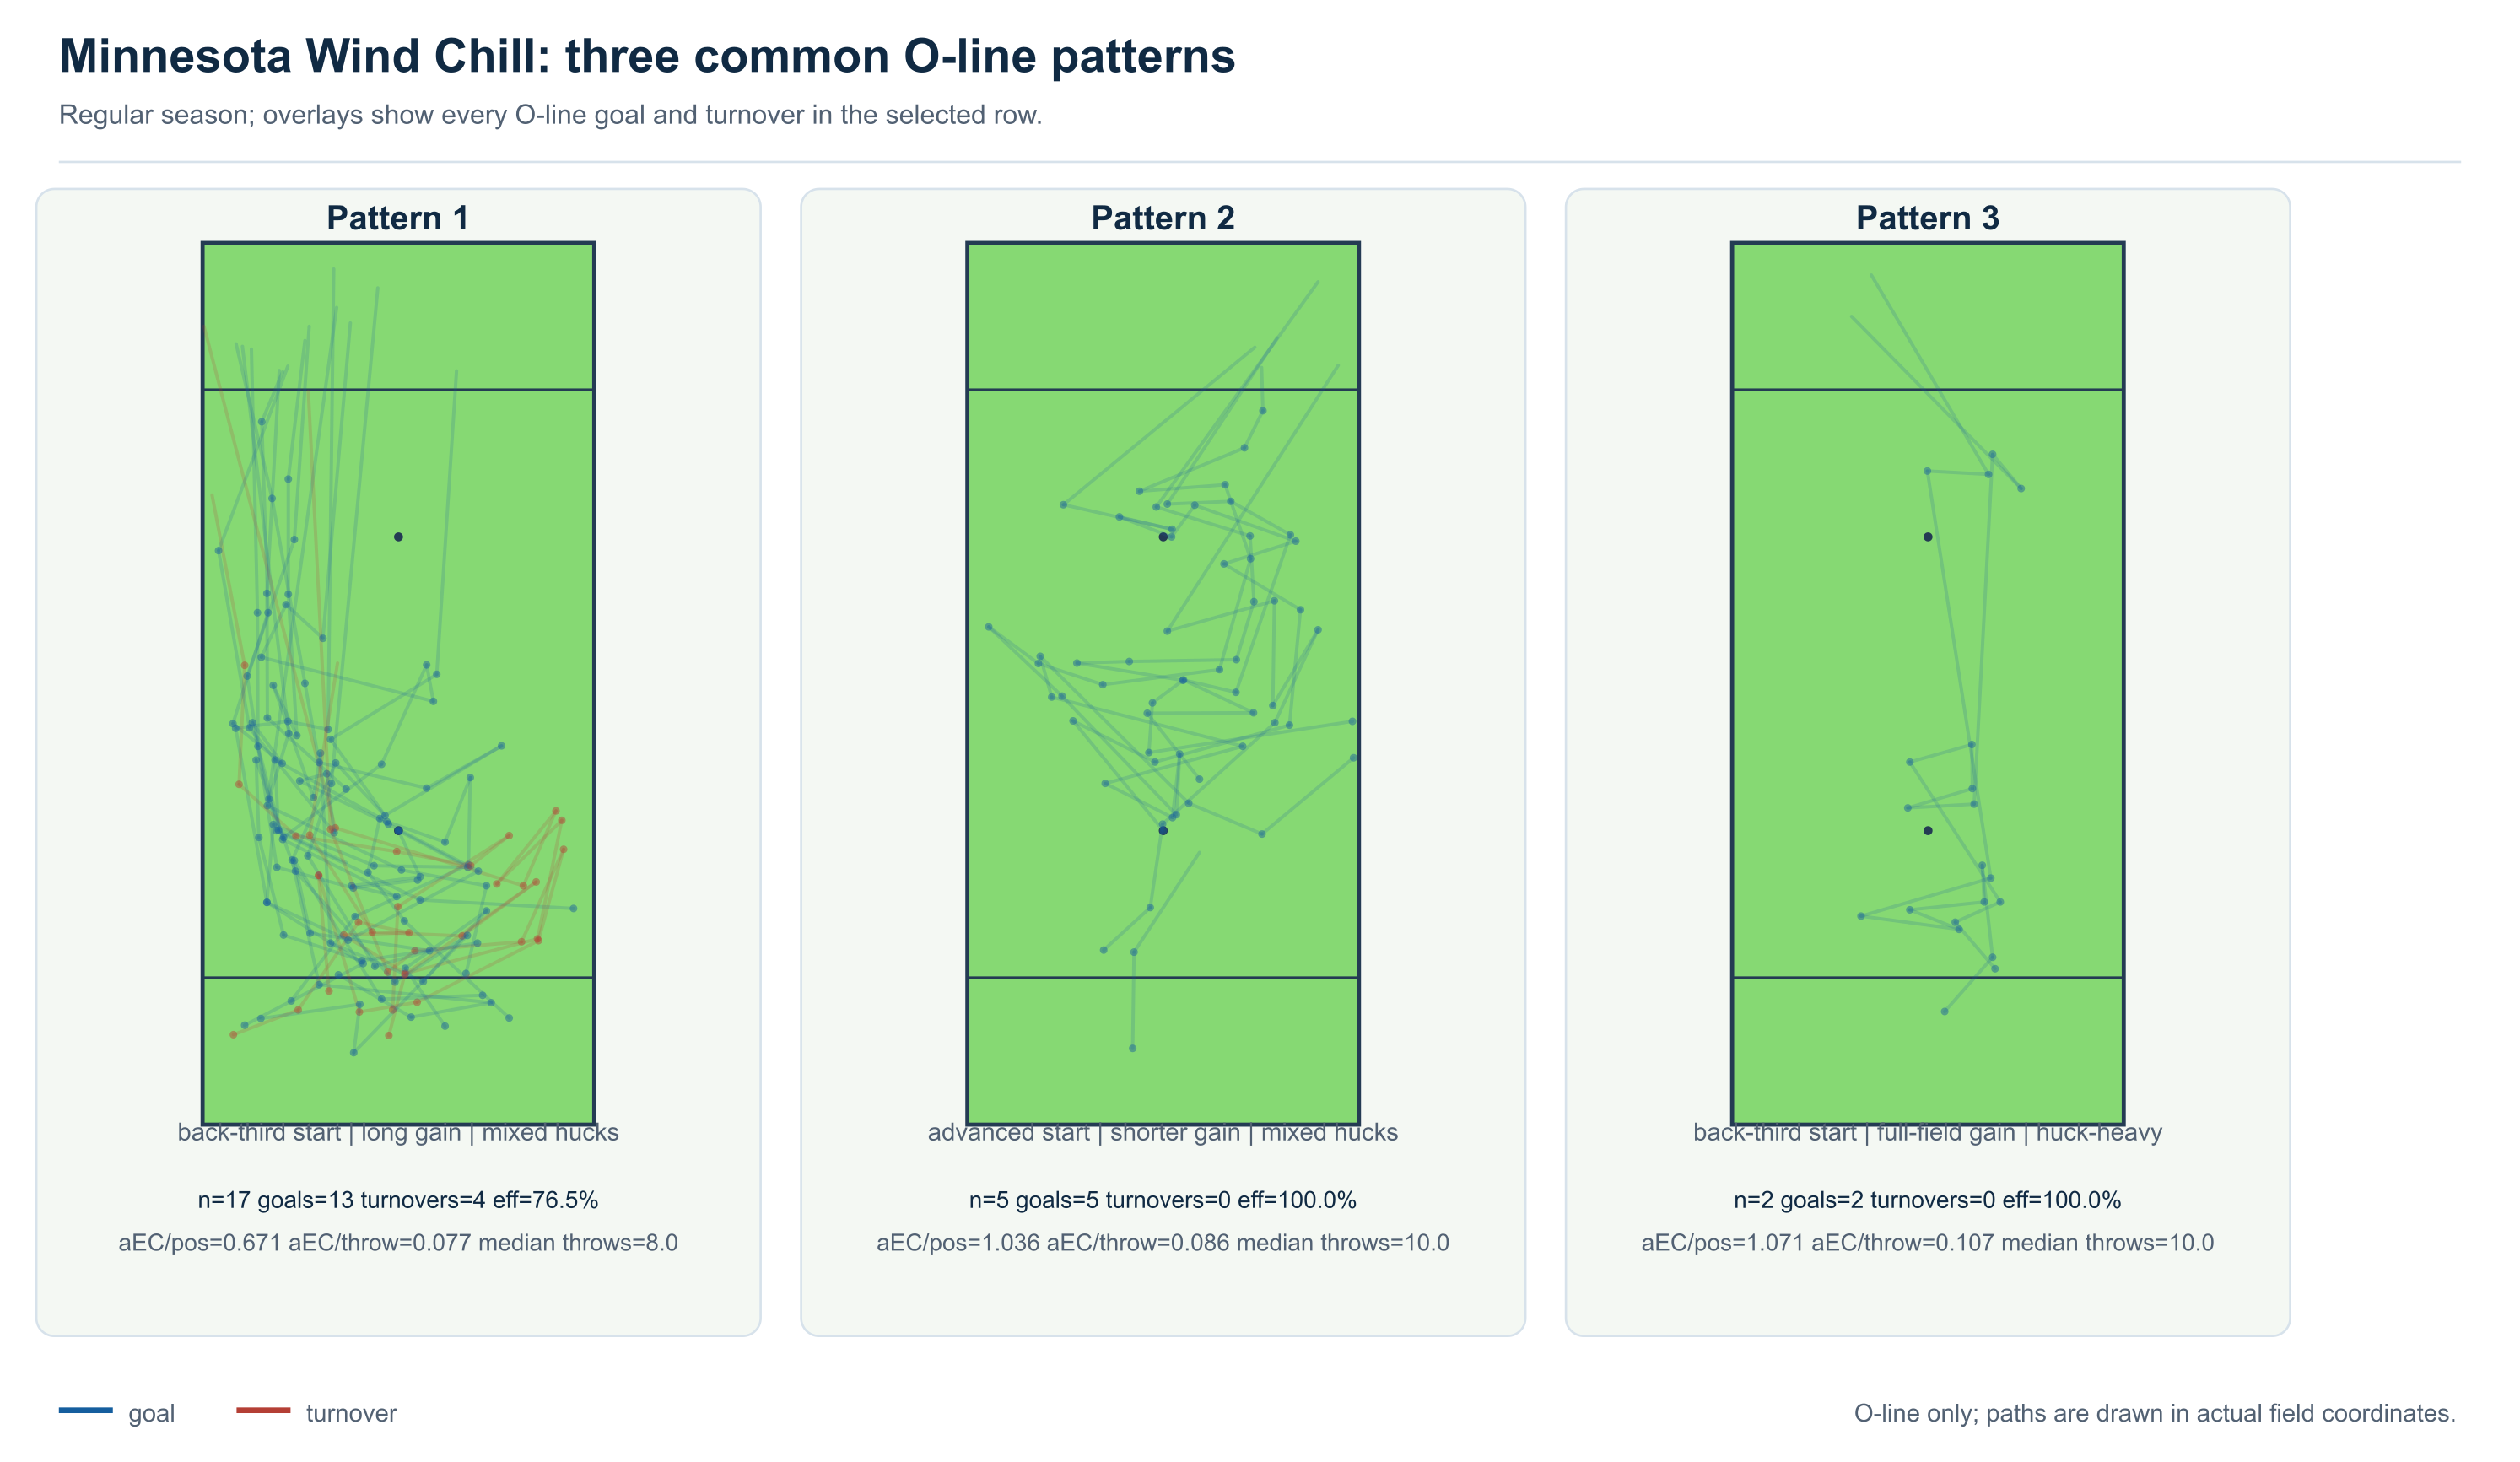
\includegraphics[width=0.98\linewidth]{generated/figures/windchill_top3_patterns.png}
  \caption{Minnesota Wind Chill's three selected recurring patterns. Pattern 3
  is deliberately shown with its small $n$ rather than being allowed to read as
  a general team tendency.}
  \label{fig:windchill}
\end{figure}

\subsection{Oakland Spiders: low-huck continuity and width}

Oakland's first two selected patterns contain no hucks at all. Pattern 1 has
eight goals and one turnover across nine possessions; Pattern 2 has 12 goals
and one turnover across 13. Their median lengths are ten and eleven throws,
respectively. Pattern 3, titled ``lateral up left sideline'' in the saved
arrangement, is shorter at an eight-throw median and converted all ten retained
possessions. Its 0.121 \aEC per throw is the highest density among Oakland's
three selected patterns.

This is a useful example of why ``small ball'' should not be confused with
``short.'' The first two Oakland patterns are low-huck, but they are not brief.
They move through a sequence of catches and throws while using the width of the
field. That reading is consistent with the public team profile, which describes
the Spiders as an offense that uses the full width of the field and pairs that
with a carefully selected deep game \citep{eberhard2026teamstrengths}. The field
overlays make the distinction visible in a way that a huck rate alone cannot.

\begin{figure}[p]
  \centering
  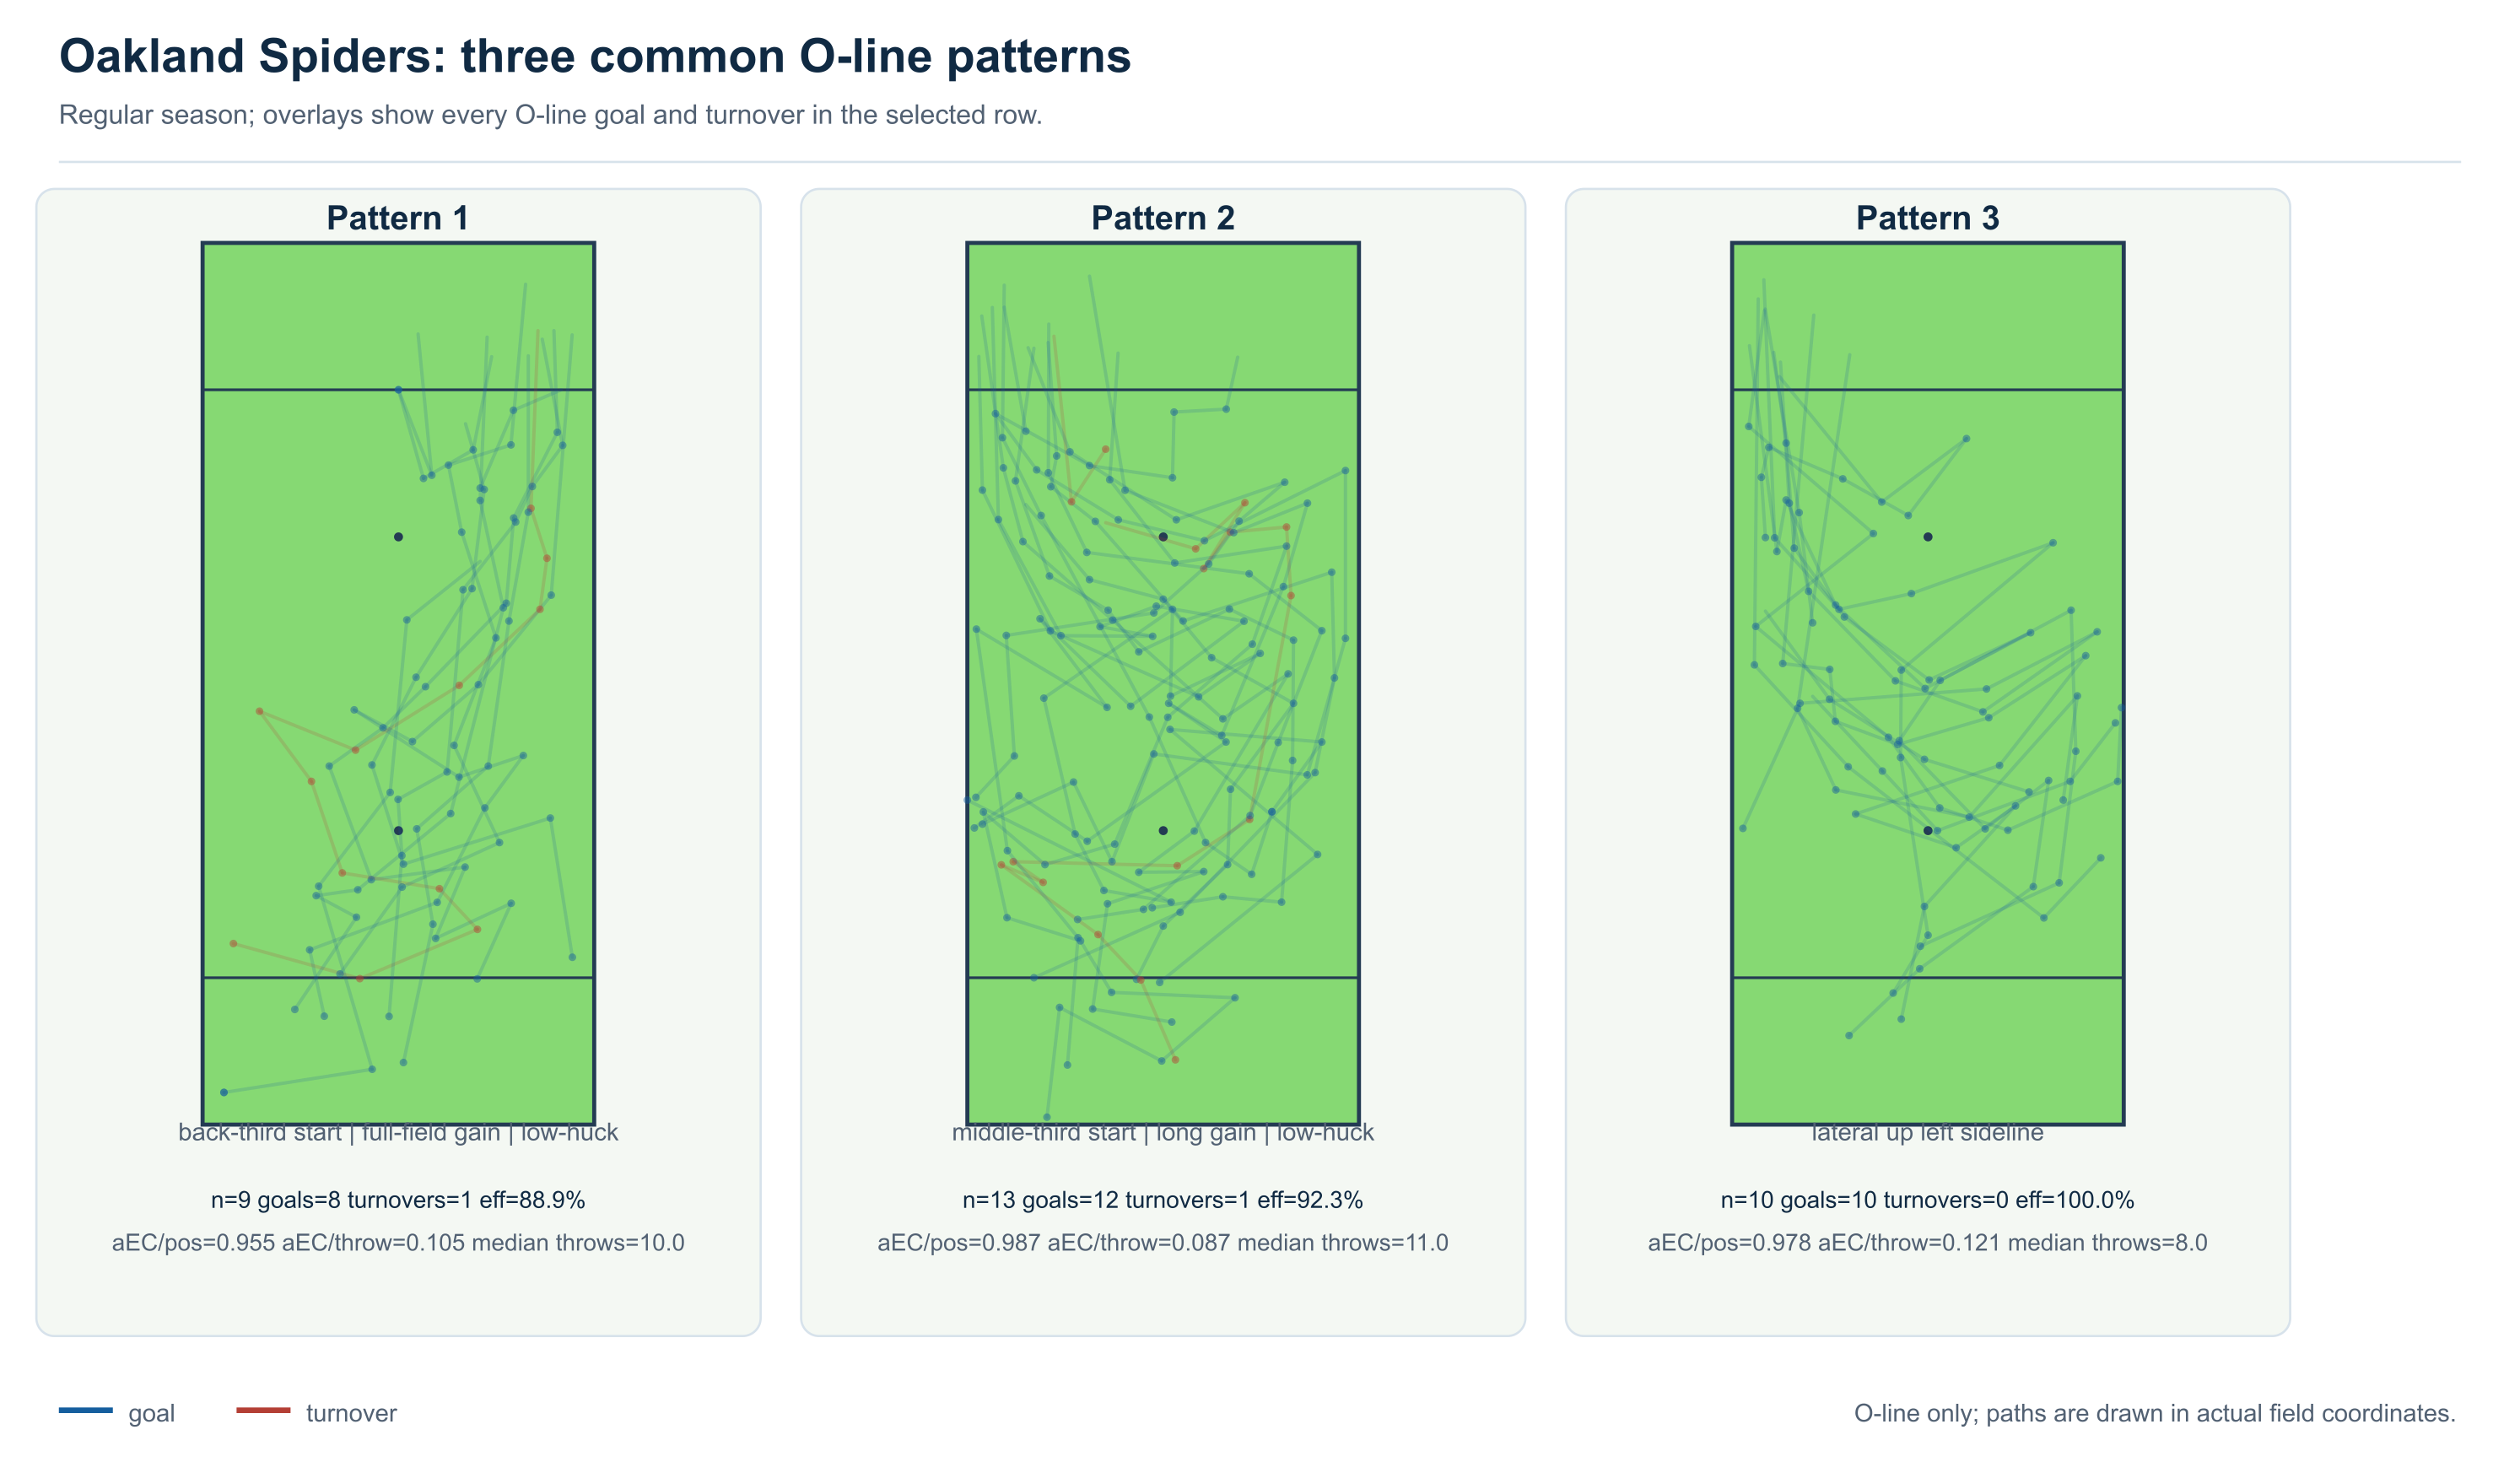
\includegraphics[width=0.98\linewidth]{generated/figures/spiders_top3_patterns.png}
  \caption{Oakland Spiders' three selected recurring patterns. The first two
  rows are low-huck, longer sequences; the third is the saved lateral-up-left-
  sideline group.}
  \label{fig:spiders}
\end{figure}

\subsection{The comparison in one table}

Table~\ref{tab:patterns} places the selected rows beside one another. The
numbers show why frequency, efficiency, and aEC should be allowed to disagree.
Empire's first row is its largest selected group, while the smaller second row
has the highest \aEC per throw in the entire four-team set. Austin's best
conversion rate belongs to its third row, not its most frequent one. Oakland's
first two groups combine strong conversion with long, low-huck sequences. And
Minnesota's two perfect rows are too small to carry the same evidentiary weight
as its 17-possession base pattern.

\begin{table}[p]
  \centering
  \caption{Metrics for the three selected patterns per focus team. Efficiency
  includes turnovers; aEC/pos. is the mean total aEC, and aEC/throw is the
  aggregate total aEC divided by aggregate throws.}
  \label{tab:patterns}
  \scriptsize
  \begin{tabular}{llrrrrrrrr}
    \toprule
    Team & Pat. & $n$ & Share & G & TO & Eff. & aEC/pos. & aEC/throw & Med. throws \\
    \midrule
    New York Empire & 1 & 25 & 9.7\% & 23 & 2 & 92.0\% & 0.914 & 0.136 & 6.0 \\
New York Empire & 2 & 11 & 4.3\% & 11 & 0 & 100.0\% & 1.000 & 0.224 & 5.0 \\
New York Empire & 3 & 6 & 2.3\% & 6 & 0 & 100.0\% & 1.049 & 0.117 & 9.0 \\
Austin Sol & 1 & 11 & 3.9\% & 8 & 3 & 72.7\% & 0.601 & 0.132 & 4.0 \\
Austin Sol & 2 & 19 & 6.7\% & 15 & 4 & 78.9\% & 0.749 & 0.069 & 10.0 \\
Austin Sol & 3 & 18 & 6.3\% & 15 & 3 & 83.3\% & 0.876 & 0.087 & 10.5 \\
Minnesota Wind Chill & 1 & 17 & 6.4\% & 13 & 4 & 76.5\% & 0.671 & 0.077 & 8.0 \\
Minnesota Wind Chill & 2 & 5 & 1.9\% & 5 & 0 & 100.0\% & 1.036 & 0.086 & 10.0 \\
Minnesota Wind Chill & 3 & 2 & 0.8\% & 2 & 0 & 100.0\% & 1.071 & 0.107 & 10.0 \\
Oakland Spiders & 1 & 9 & 3.4\% & 8 & 1 & 88.9\% & 0.955 & 0.105 & 10.0 \\
Oakland Spiders & 2 & 13 & 4.9\% & 12 & 1 & 92.3\% & 0.987 & 0.087 & 11.0 \\
Oakland Spiders & 3 & 10 & 3.8\% & 10 & 0 & 100.0\% & 0.978 & 0.121 & 8.0 \\
\bottomrule

  \end{tabular}
\end{table}

\section{Discussion}

\subsection{What the patterns add to the leaderboard}

The main contribution of these displays is interpretive rather than merely
decorative. A possession path supplies a bridge between a metric and a tactical
description. The six-passer article makes that bridge at the player level by
showing that high aEC can come from very different combinations of shooting,
volume, field vision, or support \citep{eberhard2026passers}. Here, the same
logic operates one level up. Empire's selected rows suggest several efficient
full-field solutions. Oakland's rows suggest continuity through space without
needing frequent hucks. Austin and Minnesota show how a longer possession can
be a recurring branch rather than a failure of the first option.

The distinction between total \aEC and \aEC per throw is especially useful.
Total \aEC asks how much value the entire possession accumulated. \aEC per throw
asks how concentrated that value was across the sequence. A short possession
can look excellent on the latter measure even when another longer possession
produces more total value. Neither is a universal quality score; each answers a
different question about the route.

\subsection{Turnovers change the pattern story}

If only scoring possessions were retained, several of the selected overlays
would look cleaner and several efficiency numbers would become meaningless.
Including turnovers changes the interpretation in two ways. First, it makes
``how often this pattern scores'' an observable outcome ratio rather than a
description of successful examples only. Second, it lets spatially similar
routes reveal where the same idea breaks down. The red paths in the figures are
not clutter; they are the negative evidence needed to distinguish a reliable
pattern from a memorable one.

That is also why the manuscript reports $n$ beside every percentage. A 100
percent group with two possessions is a promising observation. It is not a
league-ready estimate. The public Shown Space writing repeatedly combines
volume, efficiency, risk, and role when telling player stories
\citep{eberhard2026mvp,eberhard2026decraene}; team patterns deserve the same
discipline.

\subsection{From recurring paths to tactical language}

The current labels should remain modest. ``Lateral up left sideline'' is a
geometric description grounded in the cards. A claim such as ``Oakland always
attacks the left sideline'' would require more evidence: force direction,
opponent quality, personnel, game state, and the paths that did not score.
Likewise, a five-throw mode does not prove that a team is trying to reach five
throws. It simply identifies the most common observed length in the selected
outcome set.

The productive next step is a second manual pass. Once a team has a small set
of spatial families, an analyst can name them using both their geometry and
their function: for example, a direct deep branch, a lateral continuation
sequence, or a long reset-and-advance pattern. The figures make those judgments
auditable. Another analyst can see the same overlays, disagree with a boundary,
and revise the group without changing the underlying possession reconstruction.

\section{Limitations}

Several limitations should shape how these results are used.

First, the pattern taxonomy is analyst-curated. The three rows are useful
descriptive units, but their boundaries reflect visual judgment and the current
arrangement checkpoints. A future version should measure inter-rater agreement
or compare the manual rows with a geometry-first clustering baseline.

Second, the paper studies four teams and three selected rows per team. Large
unsorted groups remain outside the narrative by design. The figures are not a
complete description of any offense, and they should not be used to infer that
an unshown pattern is rare without checking the full browser.

Third, the sample is regular season only. It does not answer whether a team
changed its offense in the playoffs. Nor does the current summary adjust for
opponent pressure, field conditions, score state, personnel, or starting field
position. These factors can influence both the path and the outcome.

Finally, the paper uses the cached throw-level \aEC values supplied by Shown
Space; it does not refit or audit the underlying machine-learning model. The
metric is treated as a contextual contribution signal, not as a causal estimate
that a pattern alone produced the final score.

\section{Conclusion}

The four teams in this study do not reduce to a single offensive template.
Empire's selected groups combine high conversion with multiple efficient
full-field routes. Austin carries a short, aggressive branch alongside longer
sequences. Minnesota's common middle is surrounded by smaller high-value
branches whose uncertainty is visible once turnovers and sample size are shown.
Oakland's selected patterns make the strongest case for low-huck continuity:
long sequences, high conversion, and a spatial identity that depends on width
more than on constant deep shots.

The practical result is a way to write about team offense that stays close to
the field. The heatmap says how long possessions tend to last. The overlays say
where the disc travels. Efficiency and \aEC say what those routes produced.
Together they turn a possession browser into an argument about how teams build
scores, while leaving enough of the evidence visible for the reader to make a
different judgment.

\section*{Reproducibility}

All calculations and figures in this manuscript are regenerated with
\texttt{scripts/build\_paper\_figures.py}. The script reads the four saved
arrangements, filters the cached game files through July 19, 2026, writes the
CSV/LaTeX tables under \texttt{paper/generated/}, and produces standalone SVG
figures. The arrangement checkpoints remain separate from the generated
figures so later manual edits can be compared with this version. The SVG
figures are converted to the checked-in PNGs by
\texttt{scripts/render\_paper\_figures.cjs} when the figures are regenerated.

\bibliographystyle{plainnat}
\bibliography{references}

\end{document}
